%   % !TEX root = ../../VIII,3_Rahmen-TeX_8-1.tex
%
%
%   Band VIII, 3 N.~??A23/Y.3
%   Signatur/Tex-Datei: LH_35_09_16_001,020
%   RK-Nr. 41158
%   Überschrift: Explicatio mechanica elastri
%   Datierung: [Ende Januar bis März/April 1683]
%   WZ: RK-WZ 134 = Krone auf eingekreistem Ross mit Gegenmarke AB (eins)
%   SZ: (keins)
%   Bilddateien (PDF): LH_35_09_16_001,020_d1; LH_35_09_16_001,020_d2; LH_35_09_16_001,020_d3; LH_35_09_16_001,020_d4; LH_35_09_16_001,020_d5 (insgesamt: fünf)
%
%
\selectlanguage{ngerman}%
\frenchspacing%
%
\begin{ledgroupsized}[r]{120mm}
\footnotesize
\pstart
\noindent\textbf{Überlieferung:}
\pend
\end{ledgroupsized}
\begin{ledgroupsized}[r]{114mm}
\footnotesize
\pstart \parindent -6mm
\makebox[6mm][l]{\textit{L}}%
Konzept: LH~XXXV~9,~16 Bl.~1,~20.
Ein Bogen~2\textsuperscript{o};
ein Wasserzeichen auf Bl.~1 mit Gegenmarke auf Bl.~20:
Papier aus dem Harz;
% Abreibung am unteren Rand von Bl.~20 mit 
Textverlust auf Bl.~20~v\textsuperscript{o}.
Drei Seiten auf Bl.~1~v\textsuperscript{o}, 20~r\textsuperscript{o} und 20~v\textsuperscript{o};
die Überschrift befindet sich auf~Bl.~1~r\textsuperscript{o}.
Bl.~1~r\textsuperscript{o} und die ersten vier Zeilen von Bl.~1~v\textsuperscript{o} überliefern den letzten Abschnitt von N.~14\textsubscript{2} (S.~\refpassage{LH_35_09_16_001v_Ende-1}{LH_35_09_16_001v_Ende-2}),
dem N.~14\textsubscript{3} ursprünglich angeschlossen war.
\pend
\end{ledgroupsized}
%
%
% \vspace*{5mm}
% \begin{ledgroup}
% \footnotesize%
% \pstart%
% \noindent%
% \textbf{Datierungsgründe:}
% Der vorliegende Text N.~??Y\textsubscript{3} ist als Fortsetzung von N.~??A21\textsubscript{1} entstanden.
% Die Datierung von N.~??Y\textsubscript{2} wird daher übernommen.
% \pend
% \end{ledgroup}
%
\selectlanguage{latin}%
\frenchspacing%
%
%
\count\Bfootins=1100
\count\Afootins=1100
\count\Cfootins=1100
\vspace{8mm}
\pstart%
\normalsize%
\noindent%
%
\lbrack1~r\textsuperscript{o}\rbrack\
%
\pend%
\vspace{-0.5em}%
% Überschrift
\pstart%
\centering%
Explicatio Mechanica\protect\index{Sachverzeichnis}{explicatio mechanica}
Elastri\protect\index{Sachverzeichnis}{elastrum}\\
seu causa\protect\index{Sachverzeichnis}{causa restitutionis}
cur corpora\protect\index{Sachverzeichnis}{corpus tensum}
per vim\protect\index{Sachverzeichnis}{vis tendens} tensa sponte restitui videantur%
\edtext{}{%
\lemma{\textit{Am Rand:}}\Afootnote{Verte\vspace{-5mm}}}
\pend%
\vspace{0.5em}%
%
\pstart%
\noindent%
%
\lbrack1~v\textsuperscript{o}\rbrack\ % Blatt 1v
%
\edtext{Tensionis\protect\index{Sachverzeichnis}{tensio} nomine}{%
\lemma{Tensionis}\Bfootnote{%
\hspace{-0,5mm}\textbar~autem \textit{gestr.}~\textbar\ nomine%
~\textit{L}}}
%
intelligo vim quae corpori
\edtext{fit mutata figura\protect\index{Sachverzeichnis}{figura corporis}
vel volumine,\protect\index{Sachverzeichnis}{volumen corporis}}{%
\lemma{fit}\Bfootnote{%
\textit{(1)}~mutata figura aut volumine,
\textit{(2)}~mutato
\textit{(3)}~mutata \textbar~figura vel \textit{erg.}~\textbar\ volumine,%
~\textit{L}}}
%
sive diducatur
\edtext{ut chorda,\protect\index{Sachverzeichnis}{chorda diducta}}{%
\lemma{ut}\Bfootnote{%
\hspace{-0,5mm}chorda
\textit{erg.~L}}}
%
sive comprimatur ut aer,\protect\index{Sachverzeichnis}{aer compressus}
sive partim diducatur partim comprimatur,
ut baculus flexus\protect\index{Sachverzeichnis}{baculus flexus}
\edtext{cujus convexa diducuntur,}{%
\lemma{cujus}\Bfootnote{%
\textit{(1)}~exteriora di
\textit{(2)}~convexa diducuntur,%
~\textit{L}}}
%
concava comprimuntur\lbrack,\rbrack\
\edtext{modo scilicet corpus dimissum se restituat.}{%
\lemma{modo}\Bfootnote{%
\hspace{-0,5mm}scilicet \lbrack...\rbrack\ se restituat
\textit{erg.~L}}}
%
Tensio\protect\index{Sachverzeichnis}{tensio} autem ista
non tantum in corporibus\protect\index{Sachverzeichnis}{corpus tensum} illis locum habet,
ubi sensu\protect\index{Sachverzeichnis}{sensus} manifesta est,
sed in omnibus
quae sonum\protect\index{Sachverzeichnis}{sonus} edunt,
%
\edtext{sonum enim omnem a corporis\protect\index{Sachverzeichnis}{corpus percussum} percussi tensione quadam,
et secuto tremore\protect\index{Sachverzeichnis}{tremor} nasci constat.}{%
\lemma{sonum \lbrack...\rbrack\ constat}\Cfootnote{%
Siehe zu dieser Grundthese von Leibnizens Akustik die Texte N.~12\textsubscript{1} bis 12\textsubscript{3} in diesem Band.}}
%
Vitrum\protect\index{Sachverzeichnis}{vitrum flexile} ipsum flexile
\edtext{esse visu\protect\index{Sachverzeichnis}{visus} patet in}{%
\lemma{esse}\Bfootnote{%
\hspace{-0,5mm}\textbar~visu \textit{erg.}~%
\textbar\ patet
\textit{(1)}~ex
\textit{(2)}~in%
~\textit{L}}}
%
tenuibus illis filamentis\protect\index{Sachverzeichnis}{filamentum vitri}
quae ex vitro duci possunt.
Ut
\edtext{taceam experimenta\protect\index{Sachverzeichnis}{experimentum}}{%
\lemma{taceam}\Bfootnote{%
\textit{(1)}~exemplum
\textit{(2)}~experimentum
\textit{(3)}~experimenta%
~\textit{L}}}
\edtext{vitri\protect\index{Sachverzeichnis}{vitrum frigore contractum}
\edtext{frigore contracti,}{%
\lemma{frigore contracti}\Cfootnote{%
Wohl Anspielung auf einen Versuch der Accademia del Cimento \glqq circa un effetto del caldo e del freddo\grqq.
Siehe \cite{00143}L.~\textsc{Magalotti}, \textit{Saggi di naturali esperien\-ze}, Florenz 1666, S.~186.}}
% Zu diesem bei der Accademia del Cimento durchgeführten Versuch über die Dehnung und Zusammenziehung eines Gefäßes aus Kristall finden sich in \textit{LSB} VIII,~1 N.~37\cite{01100} keine Auszüge von Leibniz. Siehe jedoch seine Bemerkung (ebd. S.~283.7\textendash8\cite{01100}) zu einem ähnlichen Versuch der Florentiner Akademie.
item\protect\index{Sachverzeichnis}{vitrum sono ruptum}
\edtext{sono rupti.}{%
\lemma{sono rupti}\Cfootnote{%
Siehe % N.~??A4\textsubscript{1}, S.~\refpassage{LH_37_01_001v_VitrumMorhof-1}{LH_37_01_001v_VitrumMorhof-2} und 
N.~12\textsubscript{3}, S.~\refpassage{LH_37_01_004r_VitrumMorhof-1}{LH_37_01_004r_VitrumMorhof-2}; \refpassage{LH_37_01_008r_rv1}{LH_37_01_008r_rv2}.
Dort verweist Leibniz auf \textsc{D.\,G. Morhof}, \textit{De scypho vitreo}, 2.~Ausgabe, Kiel 1682, S.~16\,f.\cite{01207}}}}{%
\lemma{vitri}\Bfootnote{%
\textit{(1)}~soni rupti,
\textit{(2)}~item
\textit{(3)}~frigore contracti, \textbar\ item \textit{erg.} \textbar\ sono rupti.%
~\textit{L}}}
Illud solum interest,
quod dura corpora\protect\index{Sachverzeichnis}{corpus durum}
parum admodum flectuntur\protect\index{Sachverzeichnis}{corpus flexum}
et percussa,\protect\index{Sachverzeichnis}{corpus percussum}
sese velocissime restituunt;\protect\index{Sachverzeichnis}{corpus se restituens}
quemadmodum et videmus \makebox[1.0\textwidth][s]{facere chordas breves et tamen valde tensas.\protect\index{Sachverzeichnis}{chorda tensa}
Durum igitur corpus\protect\index{Sachverzeichnis}{corpus durum}
ad Usum Mechanicum\protect\index{Sachverzeichnis}{usus mechanicus}}
\pend
\newpage
\pstart
\noindent optime explicabimus,
si concipiamus tanquam constans ex
%
\edtext{fibris\protect\index{Sachverzeichnis}{fibra tensa}
sive chordis\protect\index{Sachverzeichnis}{chorda tensa} brevibus
iisque valde tensis,}{%
\lemma{fibris}\Bfootnote{\textit{(1)}~exiguis valde
\textit{(2)}~sive chordis \lbrack...\rbrack\ valde tensis% brevibus iisque 
~\textit{L}}}
%
quae si etiam tenues praeterea sint
%
\edtext{aut rariores,}{%
\lemma{aut}\Bfootnote{%
\hspace{-0,5mm}rariores \textit{erg.~L}}}
%
fragile erit;
sin crassae
%
\edtext{aut crebrae,}{%
\lemma{aut}\Bfootnote{%
\hspace{-0,5mm}crebrae \textit{erg.~L}}}
%
firmum.
Quin imo nullum arbitror in rerum natura dari
corpus\protect\index{Sachverzeichnis}{corpus perfecte durum} perfecte durum seu
\edtext{\pgrk{>'atomon,\protect\index{Sachverzeichnis}{atomus}}
quale supposuere
\edtext{quidam veteres;\protect\index{Sachverzeichnis}{veteres}}{%
\lemma{quidam veteres}\Cfootnote{%
Die Annahme vollkommen harter Atome wird von \cite{01199}\textsc{Pseudo-Plutarch}, \textit{Placita} I~3 % philosophorum Diels, Doxographi, S.~286a
besonders Epikur zugeschrieben.
Siehe hierzu \cite{01073}P.~\textsc{Gassendi}, \textit{Physica}, sectio~I, lib.~III, cap.~V (\cite{01029}\textit{GOO}~I, S.~256b\textendash257a).}}
sed nec}{%
\lemma{\pgrk{>'atomon},}\Bfootnote{%
\textit{(1)}~multo minus
\textit{(2)}~sed
\textit{(3)}~quale
\textit{(a)}~supposuit Epicuri\lbrack\textit{!}\rbrack,\protect\index{Namensregister}{\textso{Epikur} (Epicurus), um 342/1\textendash um 271/0 v.Chr.} multo minus
\textit{(b)}~supposuere quidam veteres; sed nec%
~\textit{L}}}
%
ullum esse perfecte fluidum,\protect\index{Sachverzeichnis}{corpus perfecte fluidum}
qualis est
\edtext{materia\protect\index{Sachverzeichnis}{materia subtilis} subtilis quorundam recentiorum;}{%
\lemma{materia \lbrack...\rbrack\ recentiorum}\Cfootnote{%
Siehe etwa \cite{00035}R.~\textsc{Descartes}, \textit{Principia philosophiae}, pars~II, §~66; pars~III, §~49\textendash52 (Amsterdam 1644, S.~63\textendash65, 93\textendash95; \textit{DO} VIII, 1, S.~71\textendash73; 104\,f.).}}
%
sed omnia aliquem habere gradum\protect\index{Sachverzeichnis}{gradus tenacitatis} tenacitatis,
ut non
\edtext{sine vi\protect\index{Sachverzeichnis}{vis diducens}
particulae vicinae a se invicem diduci possint,}{%
\lemma{sine}\Bfootnote{%
\hspace{-0,5mm}vi
\textit{(1)}~a se invicem
\textit{(2)}~particulae vicinae a se invicem
\textit{(a)}~removeri possint
\textit{(b)}~diduci possint,%
~\textit{L}}}
%
et eadem vi\protect\index{Sachverzeichnis}{vis cohaesionis}
\edtext{si possint}{%
\lemma{si}\Bfootnote{%
\hspace{-0,5mm}possint
\textit{erg.~L}}}
%
rursus
\edtext{conjungantur,
ea autem vis\protect\index{Sachverzeichnis}{vis cohaesionis}}{%
\lemma{conjungantur,}\Bfootnote{%
\textit{(1)}~quod
\textit{(2)}~ea autem vis%
~\textit{L}}}
%
ab
\edtext{ambientis corporis\protect\index{Sachverzeichnis}{motus corporis ambientis}
adhuc fluidioris motu\protect\index{Sachverzeichnis}{motus fluidi} petenda}{%
\lemma{ambientis}\Bfootnote{%
\textit{(1)}~fluidi mo
\textit{(2)}~subtilioris motu petendum
\textit{(3)}~corporis adhuc fluidioris motu
\textit{(a)}~petendum
\textit{(b)}~petenda%
~\textit{L}}}
%
est,
qui ea disjunctione\protect\index{Sachverzeichnis}{disjunctio} perturbatur:
\edtext{quemadmodum inde oriri dubium non est,
quod videmus fieri in duabus bullis aquae,\protect\index{Sachverzeichnis}{bulla aquae}
vel duobus orbiculis\protect\index{Sachverzeichnis}{orbiculus olei}}{%
\lemma{quemadmodum}\Bfootnote{%
\textit{(1)}~ab eo fieri
\textit{(2)}~inde oriri \lbrack...\rbrack\ in duabus
\textit{(a)}~guttis vel
\textit{(aa)}~orbicu
\textit{(bb)}~du
\textit{(b)}~bullis
\textit{(aa)}~vel
\textit{(bb)}~aquae, vel duobus orbiculis%
~\textit{L}}}
%
olei in aqua natantibus, qui
ubi se contigerint
subito in unum
\edtext{coeunt.
Item quod videmus}{%
\lemma{coeunt}\Bfootnote{%
\textit{(1)}~; quae vis eti
\textit{(2)}~. Etsi autem ea vis exigua videatur
\textit{(3)}~. Item quod videmus%
~\textit{L}}}
%
eosdem orbiculos pin-%
%  %  %  %  A C H T U N G   G E T R I X T   !  !  !  !
\edtext{}{\lemma{\hspace{1,6mm}\textit{Am Rand, auf} \lbrack\textit{Fig.~1}\rbrack\ \textit{bezogen:}}\killnumber\Afootnote{%
Man kondte 3 tropfen\protect\index{Sachverzeichnis}{tropf} oel\protect\index{Sachverzeichnis}{oel} wehlen
die auffm waßer schwimmen,
davon \textit{a} mit einem stylo\protect\index{Sachverzeichnis}{stylus} gezogen wird.\vspace{-5mm}}}%
%
%  %  %  %  A C H T U N G   G E T R I X T   !  !  !  !
\edtext{}{\lemma{\hspace{1,6mm}\lbrack\textit{Fig.~1}\rbrack}\killnumber\Cfootnote{% \hspace{1,6mm}
Der Tropfen \textit{b} im Diagramm hieß ursprünglich \textit{a}. Dies erklärt die falsche Benennung in der auf das Diagramm bezogenen Randbemerkung.}}%
%
\pend%
% \newpage%
%
%
\vspace{2em}
  \centerline{\includegraphics[width=0.36\textwidth]{gesamttex/edit_VIII,3/images/LH_35_09_16_001,020_d1.pdf}}%
  \vspace{0.0em}
  \centerline{\lbrack\textit{Fig.~1}\rbrack}%
  \label{LH_35_09_16_020r_Fig.1}%
% \vspace*{1.0em}
%künstlicher Seitenumbruch miitten im Absatz KZEITZ%%%%%%%%%%%%%%%%%%%%%%%%%%%%%%%%%%%%%%%
\newpage
\count\Bfootins=900
\count\Afootins=1000
\count\Cfootins=1000
\pstart
\noindent
guedinis\protect\index{Sachverzeichnis}{orbiculus pinguedinis}
si stylo aliquo diducantur atque oblongi reddantur,
mox dimissos se restituere
et ad rotunditatem\protect\index{Sachverzeichnis}{rotunditas}
\edtext{redire.
Cujus restitutionis causa\protect\index{Sachverzeichnis}{causa restitutionis}}{%
\lemma{redire.}\Bfootnote{%
\textit{(1)}~Quia primi
\textit{(2)}~Cujus restitutionis causa%
~\textit{L}}}
%
est,
quod circulus\protect\index{Sachverzeichnis}{circulus} est omnium figurarum\protect\index{Sachverzeichnis}{figura isoperimetra}
\edtext{isoperimetrarum \lbrack capacissima\rbrack,
sive in minimo\protect\index{Sachverzeichnis}{ambitus corporis} \lbrack ambitu\rbrack\
plurimum materiae\protect\index{Sachverzeichnis}{materia inclusa} includens,
ac proinde materiam comprehensam\protect\index{Sachverzeichnis}{materia comprehensa}
quam minimum corporis ambientis ictibus\protect\index{Sachverzeichnis}{ictus corporis ambientis} exponens.}{%
\lemma{isoperimetrarum}\Bfootnote{%
\hspace{-0,5mm}\textbar~capacissimus \textit{ändert Hrsg.}~\textbar~,
\textit{(1)}~et proinde
\textit{(2)}~sive in minimo
\textbar~ambitum \textit{ändert Hrsg.}~%
\textbar\ plurimum materiae \lbrack...\rbrack\ proinde materiam % includens, ac 
\textit{(a)}~quam minimam in medio corporis heterogenei
\textit{(b)}~ita
\textit{(c)}~comprehensam quam \lbrack...\rbrack\ ictibus exponens % minimum corporis ambientis 
\textit{(aa)}~, quoniam hoc modo minimum
\textit{(aaa)}~spat
\textit{(bbb)}~s
\textit{(ccc)}~circumferentiae occupans
\textit{(bb)}~.% Habemus%
~\textit{L}}}
%
Habemus
\edtext{}{{\xxref{LH_35_09_16_001v_hd8uz-1}{LH_35_09_16_001v_hd8uz-2}}%
\lemma{ergo}\Bfootnote{%
\textit{(1)}~originem veram vis el
\textit{(2)}~explicationem % pure Mechanicam
\textit{(3)}~explicationes pure
\textit{(a)}~Mechanicam
\textit{(b)}~Mechanicas
\textit{(aa)}~vis Elasticae
\textit{(bb)}~hujusmodi restitutionis,
\lbrack...\rbrack\ qualitatis physicae % ut minime opus sit potentiam aliquam mediam 
\textit{(aaa)}~titulo introducere
\textit{(bbb)}~occultae titulo
\lbrack...\rbrack\ surdo atque % introducere quae modo quodam
\textbar~\protect{\pgrk{>a>r<r'hzw|}} \textit{ändert Hrsg.}~\textbar\ corpora
\textit{(aaaa)}~restituat
\textit{(bbbb)}~tensa
\textit{(cccc)}~restituat; neque opus est ad \textbar~omnem \textit{erg.}~\textbar\ vim Elasticam, ut corporum volumen
\textit{(aaaaa)}~, sed
\textit{(bbbbb)}~solidum, sed
\textbar~aliquando \textit{erg.}~\textbar\ tantum ut
\lbrack...\rbrack\ potest nisi % ambitus seu superficies mutetur. Nam corpus per naturam majus minusque spatium vel volumen occupare nullo modo 
\textit{(aaaaa-a)}~parte adm
\textit{(bbbbb-b)}~extraneo admisso vel emisso. At 
\textit{(aaaaa-aa)}~majorem
\textit{(bbbbb-bb)}~majore minoreque superficie
\textit{(ccccc-cc)}~majori minorique superficiei
\lbrack...\rbrack\ ad vim % utique potest includi volumen idem, quod 
\textit{(aaaaa-aaa)}~Elasticam
\textit{(bbbbb-bbb)}~sufficit
\textit{(ccccc-ccc)}~restitutionis in quibusdam casibus sufficit.%
~\textit{L}}}%
%
\edlabel{LH_35_09_16_001v_hd8uz-1}ergo explicationes pure Mechanicas\protect\index{Sachverzeichnis}{explicatio mechanica}
hujusmodi restitutionis,\protect\index{Sachverzeichnis}{restitutio corporis}
ut minime opus sit
\edtext{potentiam\protect\index{Sachverzeichnis}{potentia media} aliquam mediam}{%
\lemma{potentiam aliquam mediam}\Cfootnote{%
Siehe etwa \cite{00044}H.~\textsc{Fabri}, \textit{Physica}, tract.~I, lib.~II, prop.~LII (Bd.~I, Lyon 1669, S.~60b).}}
%
qualitatis\protect\index{Sachverzeichnis}{qualitas physica occulta} physicae occultae titulo introducere
quae modo quodam surdo\protect\index{Sachverzeichnis}{modus surdus} atque
\lbrack\pgrk{>a>r<r'htw|}\protect\index{Sachverzeichnis}{arrhetos@\pgrk{'>a>r<rhtos}}\rbrack\
corpora restituat;
neque opus est ad omnem vim\protect\index{Sachverzeichnis}{vis elastica} Elasticam,
ut corporum volumen solidum,\protect\index{Sachverzeichnis}{volumen solidum}
sed aliquando tantum ut ambitus\protect\index{Sachverzeichnis}{ambitus corporis}
seu superficies\protect\index{Sachverzeichnis}{superficies corporis} mutetur.
Nam corpus per naturam\protect\index{Sachverzeichnis}{natura corporis}
majus minusque spatium\protect\index{Sachverzeichnis}{spatium corporis}
vel volumen\protect\index{Sachverzeichnis}{volumen corporis} occupare nullo modo potest
nisi extraneo admisso vel emisso.
At majori minorique superficiei\protect\index{Sachverzeichnis}{superficies corporis}
utique potest includi volumen idem,\protect\index{Sachverzeichnis}{volumen corporis}
quod ad vim restitutionis\protect\index{Sachverzeichnis}{vis restitutionis}
in quibusdam casibus\protect\index{Sachverzeichnis}{casus}
sufficit.\edlabel{LH_35_09_16_001v_hd8uz-2}
%
Possumus enim intelligere
\edtext{corpora quaedam se restituentia\protect\index{Sachverzeichnis}{corpus se restituens}}{%
\lemma{corpora}\Bfootnote{%
\textit{(1)}~Elastica\protect\index{Sachverzeichnis}{corpus elasticum}
\textit{(2)}~quaedam se restituentia%
~\textit{L}}}
%
ex innumeris partibus exiguis fluidis\protect\index{Sachverzeichnis}{pars corporis fluida}
\edtext{constare,
instar guttarum\protect\index{Sachverzeichnis}{gutta oblonga}
atque bullarum,\protect\index{Sachverzeichnis}{bulla oblonga}
quae vi diducentis\protect\index{Sachverzeichnis}{vis diducens} aut comprimentis\protect\index{Sachverzeichnis}{vis comprimens}
fiunt oblongae;}{%
\lemma{constare,}\Bfootnote{%
\textit{(1)}~quae
\textit{(2)}~instar guttarum \lbrack...\rbrack\ quae vi % atque bullarum,
\textit{(a)}~trahentis aut
\textit{(b)}~diducentis aut comprimentis fiunt
\textit{(aa)}~obliquae
\textit{(bb)}~oblongae;%
~\textit{L}}}
%
at dimissae redeunt ad figuram orbicularem.\protect\index{Sachverzeichnis}{figura orbicularis}
%
%%  %  %  %  A C H T U N G   G E T R I X T   !  !  !  !
%\edtext{}{\lemma{\hspace{1,6mm}\textit{Am Rand, auf} \lbrack\textit{Fig.~1}\rbrack\ \textit{bezogen:}}\killnumber\Afootnote{%
%Man kondte 3 tropfen\protect\index{Sachverzeichnis}{tropf} oel\protect\index{Sachverzeichnis}{oel} wehlen
%die auffm waßer schwimmen,
%davon \textit{a} mit einem stylo\protect\index{Sachverzeichnis}{stylus} gezogen wird.}}%
%%
%%  %  %  %  A C H T U N G   G E T R I X T   !  !  !  !
%\edtext{}{\lemma{\lbrack\textit{Fig.~1}\rbrack}\killnumber\Cfootnote{% \hspace{1,6mm}
%Der Tropfen \textit{b} im Diagramm hieß ursprünglich \textit{a}. Dies erklärt die falsche Benennung in der auf das Diagramm bezogenen Randbemerkung.}}%
%%
\pend%
%% \newpage%
%%
%%
%\vspace*{2.0em}
%  \centerline{\includegraphics[width=0.36\textwidth]{gesamttex/edit_VIII,3/images/LH_35_09_16_001,020_d1.pdf}}%
%  \vspace*{0.0em}
%  \centerline{\lbrack\textit{Fig.~1}\rbrack}%
%  \label{LH_35_09_16_020r_Fig.1}%
%% \vspace*{1.0em}
\pstart%
Cohaeret\edlabel{LH_35_09_16_001v_tabpol-1}
%
%  %  %  %  A C H T U N G   G E T R I X T   !  !  !  !
% \edtext{}{\lemma{\hspace{1,6mm}\textit{Am Rand, auf} \lbrack\textit{Fig.~1}\rbrack\ \textit{bezogen:}}\killnumber\Afootnote{%
% man kondte 3 tropfen\protect\index{Sachverzeichnis}{tropf} oel\protect\index{Sachverzeichnis}{oel} wehlen
% die auffm waßer schwimmen
% davon \textit{a} mit einem stylo\protect\index{Sachverzeichnis}{stylus} gezogen wird.}}
%
autem una gutta\protect\index{Sachverzeichnis}{gutta olei} alteri,
ex eo principio\protect\index{Sachverzeichnis}{principium}
\edtext{quo Tabulae\protect\index{Sachverzeichnis}{tabulae politae} duae}{%
\lemma{quo}\Bfootnote{%
\textit{(1)}~Tabula una
\textit{(2)}~Tabulae duae%
~\textit{L}}}
%
politae in loco clauso\protect\index{Sachverzeichnis}{locus clausus}
pleno;\protect\index{Sachverzeichnis}{locus plenus}
de
\edtext{quo
\edtext{alias}{%
\lemma{alias}\Cfootnote{% Siehe 
N.~14\textsubscript{2}, S.~\refpassage{LH_37_03_069r_duaetabulae-1}{LH_37_03_069r_duaetabulae-2}
und N.~14\textsubscript{5}, S.~\refpassage{LH037_03_118r_wiedergabe-1}{LH037_03_118r_wiedergabe-2}.}}
diximus.
Quilibet autem}{%
\lemma{quo}\Bfootnote{\hspace{-0,5mm}%
\textit{(1)}~supra
\textit{(2)}~alias diximus.
\textit{(a)}~Totus autem
\textit{(b)}~Quilibet autem%
~\textit{L}}}
%
locus mundi\protect\index{Sachverzeichnis}{mundus} haberi potest
pro clauso\protect\index{Sachverzeichnis}{locus clausus} et pleno,\protect\index{Sachverzeichnis}{locus plenus}
et duae guttae\protect\index{Sachverzeichnis}{gutta olei} se semper contingent non quidem in puncto,
sed in aliquo tractu,
\makebox[1.0\textwidth][s]{ubi perfecte satis applicatae\protect\index{Sachverzeichnis}{guttae sibi applicatae} sibi possunt 
%
\edtext{intelligi.\edlabel{LH_35_09_16_001v_tabpol-2}
\edtext{Ponamus ergo versus \textit{a} trahi guttam \textit{b}.%
}{\lemma{Ponamus \lbrack...\rbrack\ guttam \textit{b}}\Cfootnote{%
Siehe das Diagramm \lbrack\textit{Fig.~1}\rbrack\ auf S.~\pageref{LH_35_09_16_020r_Fig.1}.}}}{%
\lemma{intelligi.}\Bfootnote{%
\textit{(1)}~Ponamus er
\textit{(2)}~Ponamus ergo
\textit{(a)}~guttam \textit{a} trahi
\textit{(b)}~versus \textit{a} trahi guttam \textit{b}.%
~\textit{L}}}}
%
\pend
\newpage
\pstart
\noindent
Ea cum osculetur guttam \textit{c}
quantulocunque velut labio,\protect\index{Sachverzeichnis}{labium}
ab ea non statim divelletur,
\edtext{sed eam}{%
\lemma{sed}\Bfootnote{%
\textit{(1)}~gutta
\textit{(2)}~eam%
~\textit{L}}}
%
secum trahere conabitur,
et haec vicissim guttam\protect\index{Sachverzeichnis}{gutta olei} \textit{d}
quam
%
\edtext{ponamus parieti\protect\index{Sachverzeichnis}{paries} immobili~\textit{e} adhaerere osculo\protect\index{Sachverzeichnis}{osculum} aliquo,
is}{%
\lemma{ponamus}\Bfootnote{%
\textit{(1)}~mobili
\textit{(2)}~parieti immobili~\textit{e} adhaerere
\textbar~osculo aliquo, \textit{erg.}~\textbar\
\textit{(a)}~qui
\textit{(b)}~is%
~\textit{L}}}
%
ergo cum sequi non possit,
retineatque guttam \textit{d},
\edtext{ideo guttae\protect\index{Sachverzeichnis}{gutta olei}}{%
\lemma{ideo}\Bfootnote{% 
\hspace{-0,5mm}guttae
\textit{erg.~L}}}
%
omnes antequam a se invicem divellantur,
oblongae\protect\index{Sachverzeichnis}{gutta oblonga} fient,
idque tamdiu donec
\edtext{vis\protect\index{Sachverzeichnis}{vis divellens}
materiae ambientis\protect\index{Sachverzeichnis}{materia ambiens}
(\protect\vphantom)quae}{%
\lemma{vis}\Bfootnote{%
\textit{(1)}~quae
\textit{(2)}~materiae ambientis (\protect\vphantom)quae%
~\textit{L}}}
%
dilatationi\protect\index{Sachverzeichnis}{dilatatio guttae} earum resistit,
et, ob crescentem continue dilatationem,\protect\index{Sachverzeichnis}{dilatatio guttae}
seu superficiem quam occupant,\protect\index{Sachverzeichnis}{superficies guttae}
etiam continue crescit\protect\vphantom()
\edtext{major fiat quam vis\protect\index{Sachverzeichnis}{vis cohaesionis}}{%
\lemma{major}\Bfootnote{%
\textit{(1)}~vis
\textit{(2)}~fiat quam vis%
~\textit{L}}}
%
qua
\edtext{earum labia\protect\index{Sachverzeichnis}{labium} cohaerent,}{%
\lemma{earum}\Bfootnote{%
\textit{(1)}~oscula co
\textit{(2)}~labia cohaerent,%
~\textit{L}}}
%
quae semper eadem permanet,
aut certe non major, sed potius
\edtext{osculis\protect\index{Sachverzeichnis}{osculum} diductis,}{%
\lemma{osculis}\Bfootnote{%
\hspace{-0,5mm}diductis,
\textit{erg.~L}}}
%
minor fit.
Tunc ergo guttae\protect\index{Sachverzeichnis}{gutta olei} a se invicem divelluntur.
\edtext{Unde manifestum est ad explicandam corporum firmitatem\protect\index{Sachverzeichnis}{firmitas corporis}}{%
\lemma{Unde}\Bfootnote{%
\textit{(1)}~intelligi
\textit{(2)}~manifestum est ad explicandam
\textit{(a)}~rerum fi
\textit{(b)}~corporum firmitatem%
~\textit{L}}}
%
atque cohaesionem\protect\index{Sachverzeichnis}{cohaesio corporis}
non esse opus atomis,\protect\index{Sachverzeichnis}{atomus}
figurisque eorum hamatis\protect\index{Sachverzeichnis}{figura hamata}
atque uncinatis,\protect\index{Sachverzeichnis}{figura uncinata}
imo nec opus
\edtext{esse semper particulis ramosis\protect\index{Sachverzeichnis}{particula ramosa} 
atque filamentis implexis,\protect\index{Sachverzeichnis}{filamentum implexum}
cum}{%
\lemma{esse}\Bfootnote{%
\textit{(1)}~ramosis
\textit{(2)}~semper particulis ramosis atque
\textit{(a)}~intectis
\textit{(b)}~\textbar\ filamentis \textit{erg.} \textbar\ implexis,
\textit{(aa)}~sed
\textit{(bb)}~cum%
~\textit{L}}}
%
rursus quaeri
\edtext{possit unde}{%
\lemma{possit}\Bfootnote{%
\textit{(1)}~cur
\textit{(2)}~unde%
~\textit{L}}}
%
unci\protect\index{Sachverzeichnis}{uncus} illi atomorum\protect\index{Sachverzeichnis}{atomus}
%
\lbrack20~r\textsuperscript{o}\rbrack\ % Blatt 20r
%
suam firmitatem,\protect\index{Sachverzeichnis}{firmitas atomi}
ramique\protect\index{Sachverzeichnis}{ramus}
aut filamenta\protect\index{Sachverzeichnis}{filamentum implexum} suam habeant
\edtext{tenacitatem;\protect\index{Sachverzeichnis}{tenacitas}
videmus enim firmitatem\protect\index{Sachverzeichnis}{firmitas corporis}
ultima analysi\protect\index{Sachverzeichnis}{analysis ultima}
revocari posse ad simplicissimum}{%
\lemma{tenacitatem;}\Bfootnote{%
\textit{(1)}~sed
\textit{(a)}~simplicis
\textit{(b)}~ultima firmitatis analysi
\textit{(2)}~sed
\textit{(3)}~videmus
\textbar~enim \textit{erg.}~%
\textbar\ firmitatem ultima \lbrack...\rbrack\ ad simplicissimum%
~\textit{L}}}
%
naturae artificium,\protect\index{Sachverzeichnis}{artificium naturae}
\edtext{guttas,\protect\index{Sachverzeichnis}{gutta olei}
aut si cavae\protect\index{Sachverzeichnis}{gutta cava} sint,
bullas\protect\index{Sachverzeichnis}{bulla} sibi invicem apponentis,}{%
\lemma{guttas,}\Bfootnote{%
\textit{(1)}~quae si
\textit{(2)}~aut si cavae sint,
\textit{(a)}~bullas
\textit{(b)}~bullas sibi invicem
\textit{(aa)}~ad eo
\textit{(bb)}~annectentis
\textit{(cc)}~apponentis,%
~\textit{L}}}
%
ex quibus
\edtext{in longum ordinatis paulatim}{%
\lemma{quibus}\Bfootnote{%
\hspace{-0,5mm}\textbar~in longum ordinatis \textit{erg.}~\textbar\
\textit{(1)}~sibi
\textit{(2)}~paulatim%
~\textit{L}}}
%
filamenta\protect\index{Sachverzeichnis}{filamentum implexum}
\edtext{ducuntur,
et ex his fibrae\protect\index{Sachverzeichnis}{fibra} texuntur.}{%
\lemma{ducuntur,}\Bfootnote{%
\textit{(1)}~aut fibrae texuntur.
\textit{(2)}~et ex his fibrae texuntur.%
~\textit{L}}}
%
\edtext{%
Guttas autem ipsas connectit et format ipsa
\lbrack earum\rbrack\
heterogeneitas ab ambiente\protect\index{Sachverzeichnis}{heterogeneitas ab ambiente}
seu materiae ex qua conflantur
a materia in qua conflantur diversitas\protect\index{Sachverzeichnis}{diversitas materiae}
secundum crassitiem\protect\index{Sachverzeichnis}{crassities materiae}
et subtilitatem.\protect\index{Sachverzeichnis}{subtilitas materiae}}{%
\lemma{Guttas}\Bfootnote{%
\hspace{-0,5mm}autem \lbrack...\rbrack\ format ipsa % ipsas connectit et
\textbar~eorum \textit{ändert Hrsg.}~%
\textbar\ heterogeneitas
\textit{(1)}~seu diversitas materiae
\textit{(2)}~ab ambiente seu
\textit{(a)}~diversitas
\textit{(b)}~materiae ex \lbrack...\rbrack\ a materia % qua conflantur
\textit{(aa)}~unde
\textit{(bb)}~in qua \lbrack...\rbrack\ et subtilitatem. % conflantur diversitas secundum crassitiem 
\textit{erg.~L}}}
%
Quodsi cavae sint guttae,\protect\index{Sachverzeichnis}{gutta cava}
id est si sint
\edtext{bullae,\protect\index{Sachverzeichnis}{bulla oblonga}
etiam materia\protect\index{Sachverzeichnis}{materia inclusa} 
inclusa oblongitati}{%
\lemma{bullae,}\Bfootnote{%
\hspace{-0,5mm}\textbar~etiam \textit{erg.}~%
\textbar\ materia inclusa
\textbar~etiam \textit{gestr.}~%
\textbar\ oblongitati%
~\textit{L}}}
%
bullarum\protect\index{Sachverzeichnis}{bulla oblonga} renititur,
quoniam
\edtext{ita libere}{%
\lemma{ita}\Bfootnote{%
\hspace{-0,5mm}\textbar~compressa \textit{gestr.}~\textbar\ libere%
~\textit{L}}}
%
satis
\edtext{atque aequabiliter}{%
\lemma{atque}\Bfootnote{%
\hspace{-0,5mm}aequabiliter
\textit{erg.~L}}}
%
moveri intus non potest,
atque
\edtext{}{{\xxref{KZeitz175}{KZeitz176}}%
{%
\lemma{proinde}\Bfootnote{%
\textit{(1)}~renisus ille
\textit{(2)}~resistent
\textit{(3)}~resistentia illa
\textit{(a)}~tam ab exter
\textit{(b)}~tam a materia
\textit{(aa)}~sive
\textit{(bb)}~exteriorem convexam,
\textit{(aaa)}~sive
\textit{(bbb)}~quam interiorem concavam superficiem ambiente%
~\textit{L}}}}%
\edlabel{KZeitz175}proinde resistentia\protect\index{Sachverzeichnis}{resistentia a materia} illa
tam a materia exteriorem convexam,
quam \makebox[1.0\textwidth][s]{interiorem concavam superficiem ambiente\protect\index{Sachverzeichnis}{materia ambiens}\edlabel{KZeitz176}
%
peti potest.
Fieri etiam potest ut guttulae\protect\index{Sachverzeichnis}{gutta tensa}}
\pend
\newpage
\pstart
\noindent
\edtext{illae jam tensae atque
in situ \lbrack oblongo\rbrack\ deprehensae,}{%
\lemma{illae}\Bfootnote{%
\textit{(1)}~tensae
\textit{(2)}~jam tensae atque in
\textbar~illo \textit{gestr.}~%
\textbar\ situ
\textbar~obliquo \textit{ändert Hrsg.}~%
\textbar\ deprehensae,%
~\textit{L}}}
%
congelentur atque
\edtext{obrigescant,
cum scilicet motus partium\protect\index{Sachverzeichnis}{motus partium}
ex quibus ipsae guttae\protect\index{Sachverzeichnis}{gutta tensa} conflatae sunt,
fit lentior;}{%
\lemma{obrigescant,}\Bfootnote{%
\textit{(1)}~aut etiam ut
\textit{(a)}~cesset
\textit{(b)}~fluidum ambiens
\textit{(2)}~sive quod motus
\textit{(3)}~cum scilicet \lbrack...\rbrack\ fit lentior;%
~\textit{L}}}
%
vel etiam fieri
\edtext{potest
ut tensioni\protect\index{Sachverzeichnis}{tensio} tali assuescant,
quemadmodum videmus multa Elastra\protect\index{Sachverzeichnis}{elastrum tensum} diu tensa}{%
\lemma{potest}\Bfootnote{%
\textit{(1)}~tensi
\textit{(2)}~ut
\textit{(a)}~aliquandiu in situ tensionis m
\textit{(b)}~ten
\textit{(c)}~tensioni tali \lbrack...\rbrack\ diu tensa% % assuescant, quemadmodum videmus multa Elastra
~\textit{L}}}
%
vim\protect\index{Sachverzeichnis}{vis elastica} Elasticam amittere,
quoniam fluidum ambiens\protect\index{Sachverzeichnis}{fluidum ambiens}
paulatim se quoque novis meatibus,\protect\index{Sachverzeichnis}{meatus}
et novos meatus sibi accommodat.
Hoc facto imposterum situs\protect\index{Sachverzeichnis}{situs oblongus}
\edtext{ille oblongus}{%
\lemma{ille}\Bfootnote{%
\textit{(1)}~obliqu
\textit{(2)}~oblongus%
~\textit{L}}}
%
guttarum\protect\index{Sachverzeichnis}{gutta oblonga}
vel bullarum\protect\index{Sachverzeichnis}{bulla oblonga}
habendus erit pro naturali\protect\index{Sachverzeichnis}{situs naturalis}
et si ab eo dimoveantur longiusque extendantur,
ac magis
\edtext{fiant % \edlabel{e020r1} \edlabel{e020r2} {\xxref{e020r1}{e020r2}}
\lbrack oblongae\rbrack,
et si ad rotunditatem\protect\index{Sachverzeichnis}{rotunditas} revocentur
id quoque tensio\protect\index{Sachverzeichnis}{tensio} erit.}{%
\lemma{fiant}\Bfootnote{%
\hspace{-0,5mm}\textbar~obliquae, \textit{ändert Hrsg.}~\textbar\
\textit{(1)}~id tensio erit
\textit{(2)}~vel ad remo
\textit{(3)}~et si \lbrack...\rbrack\ id quoque % ad rotunditatem revocentur,
\textit{(a)}~erit
\textit{(b)}~tensio erit.%
~\textit{L}}}
\pend%
\vspace{1.0em}%
% \newpage%
%
\pstart%
\noindent%
\lbrack\textit{Nachfolgend kleingedruckter Text in L gestrichen:}\rbrack\
\pend%
%
\pstart%
\footnotesize
\noindent%
Si jam ponamus guttam aliquam,
ut olei,\protect\index{Sachverzeichnis}{gutta olei}
in corpore heterogeneo,\protect\index{Sachverzeichnis}{corpus heterogeneum}
ut aqua,\protect\index{Sachverzeichnis}{aqua}
positam turbare in ratione superficiei,\protect\index{Sachverzeichnis}{superficies guttae}
adeoque vim qua gutta olei ${\scriptstyle\textit{1}}a$ tensa est\protect\index{Sachverzeichnis}{gutta tensa}
usque in ${\scriptstyle\textit{2}}a,$
esse ad vim qua tensa est\protect\index{Sachverzeichnis}{vis tendens}
usque
\edtext{in ${\scriptstyle\textit{3}}a$ ut}{%
\lemma{in}\Bfootnote{%
\hspace{-0,5mm}${\scriptstyle\textit{3}}a$
\textit{(1)}~esse
\textit{(2)}~ut%
~\textit{L}}}
%
superficies guttae ${\scriptstyle\textit{2}}a$
ad superficiem
\edtext{guttae ${\scriptstyle\textit{3}}a;$
sitque}{%
\lemma{guttae}\Bfootnote{%
\hspace{-0,5mm}${\scriptstyle\textit{3}}a;$
\textit{(1)}~sintque
\textit{(2)}~sitque%
~\textit{L}}}
%
porro superficies guttae\protect\index{Sachverzeichnis}{superficies guttae}
{\normalsize{\lbrack\textit{Text bricht ab.}\rbrack}}
\pend%
% \newpage%
%
%
\vspace{1em}
  \centerline{\includegraphics[width=0.18\textwidth]{gesamttex/edit_VIII,3/images/LH_35_09_16_001,020_d2.pdf}}%
  \vspace{0.5em}
  \centerline{\lbrack\textit{Fig.~2, gestr.}\rbrack}% \footnotesize{}
  \label{LH_35_09_16_020r_Fig.2}%
 \vspace{1.5em}
%\newpage%
%
%
\pstart%
Aliis multis modis explicari potest vis Elastica,\protect\index{Sachverzeichnis}{vis elastica}
sed omnium principium\protect\index{Sachverzeichnis}{principium} commune est,
\edtext{motus\protect\index{Sachverzeichnis}{motus partium} partium fluidi\protect\index{Sachverzeichnis}{fluidum ambiens}}{%
\lemma{motus}\Bfootnote{%
\textit{(1)}~fluidi
\textit{(2)}~partium fluidi%
~\textit{L}}}
%
varius\protect\index{Sachverzeichnis}{motus varius} et concitatus,\protect\index{Sachverzeichnis}{motus concitatus}
illi similis,
qui in meditullio aquae\protect\index{Sachverzeichnis}{aqua fervens} igni supposito\protect\index{Sachverzeichnis}{ignis suppositus} ferventis
\edtext{aut baculo\protect\index{Sachverzeichnis}{baculus} fortiter agitatae\protect\index{Sachverzeichnis}{aqua agitata}
oculis\protect\index{Sachverzeichnis}{oculus} ipsis notari potest,
si qua corpuscula\protect\index{Sachverzeichnis}{corpusculum} levia per aquam transparentem visibilia
in ea sursum deorsum innumerabilibus modis ferri concipiantur.
Si enim}{%
\lemma{aut}\Bfootnote{%
\textit{(1)}~fortiter agitat
\textit{(2)}~baculo fortiter agitatae
\textbar~oculis ipsis \textit{erg.}~%
\textbar\ notari potest,
\textit{(a)}~is enim
\textit{(b)}~si qua \lbrack...\rbrack\ sursum deorsum % corpuscula levia per aquam transparentem visibilia in ea
\textit{(aa) }ferri, atque
\textit{(bb)}~innumerabilibus modis ferri
\textit{(aaa)}~conspiciantur
\textit{(bbb)}~concipiantur. Si enim%
~\textit{L}}}
%
corpus\protect\index{Sachverzeichnis}{corpus crassum} aliquod in tali fluido reperiatur,
quod sit
\edtext{crassius ipso}{%
\lemma{crassius}\Bfootnote{%
\textit{(1)}~quam
\textit{(2)}~ipso%
~\textit{L}}}
%
\makebox[1.0\textwidth][s]{fluido,\protect\index{Sachverzeichnis}{fluidum ambiens}
\edtext{neque in partes\protect\index{Sachverzeichnis}{pars corporis}
tam minutas sese dividi patiatur,}{%
\lemma{neque}\Bfootnote{%
\textit{(1)}~easdem divisiones
\textit{(2)}~in
\textit{(a)}~partes 
\textit{(b)}~partes tam \lbrack...\rbrack\ dividi patiatur,%
~\textit{L}}}
%
in quas ipsum fluidum disper-}
\pend
\newpage
\pstart
\noindent gitur,
\edtext{id partes fluidi}{%
\lemma{id}\Bfootnote{%
\textit{(1)}~necessario fl
\textit{(2)}~motui ipsius
\textit{(3)}~partes fluidi%
~\textit{L}}}
%
sese minores et in se incurrentes, repellit,
neque se ab illis statim in diversa
\edtext{detrahi comminuique patitur;}{%
\lemma{detrahi}\Bfootnote{%
\textit{(1)}~patitur
\textit{(2)}~comminuique patitur;%
~\textit{L}}}
%
ac proinde necessario motum fluidi\protect\index{Sachverzeichnis}{motus fluidi} turbat,
\edtext{unde sequitur,}{%
\lemma{unde}\Bfootnote{%
\textit{(1)}~necesse est
\textit{(2)}~sequitur,%
~\textit{L}}}
%
ut vel plane a fluido\protect\index{Sachverzeichnis}{fluidum ambiens} expellatur,
vel ab eo comprimatur in minimum spatium,\protect\index{Sachverzeichnis}{spatium minimum}
aut certe minimam superficiem\protect\index{Sachverzeichnis}{superficies minima}
cujus capax est,
ut quam minimum
\edlabel{LH_35_09_16_020r_wdar-3}turbet.
Et quia fluidum ambiens\protect\index{Sachverzeichnis}{fluidum ambiens}
corporis interspersi\protect\index{Sachverzeichnis}{corpus interspersum}
partes\protect\index{Sachverzeichnis}{pars corporis} dissipare conatur,
multo magis discretas jam aut flexiles a se invicem dimovebit\lbrack,\rbrack\
ut sint rarae nantes in gurgite\protect\index{Sachverzeichnis}{gurges} vasto
magnosque inter se
pro liberiore \lbrack ipsarummet\rbrack\ gyratione\protect\index{Sachverzeichnis}{gyratio}
et fluidi intercurrentis motu,\protect\index{Sachverzeichnis}{motus fluidi}
meatus\protect\index{Sachverzeichnis}{meatus fluidi} relinquant,
in quo consistit corporum rarefactio\protect\index{Sachverzeichnis}{rarefactio}
sive dilatatio,\protect\index{Sachverzeichnis}{dilatatio}
et vicissim condensatio\protect\index{Sachverzeichnis}{condensatio}
sive compressio,\protect\index{Sachverzeichnis}{compressio}
et causa\protect\index{Sachverzeichnis}{causa dilatationis}\protect\index{Sachverzeichnis}{causa compressionis}
cur majus minusque spatium
(\protect\vphantom)%
in speciem\protect\index{Sachverzeichnis}{species} saltem%
\protect\vphantom()
occupare affectent.
Quanquam non omnes quod occupant impleant.
Atque hinc habetur origo mechanica\protect\index{Sachverzeichnis}{origo mechanica}
% PERLE: \protect\index{Sachverzeichnis}{mechanica fluidi}
fluidi alicujus\protect\index{Sachverzeichnis}{fluidum elasticum}
\edlabel{LH_35_09_16_020r_wdar-4}Elastici,%
\edtext{}{%
{\xxref{LH_35_09_16_020r_wdar-3}{LH_35_09_16_020r_wdar-4}}%
\lemma{turbet.}\Bfootnote{%
\textit{(1)}~Ex his possumus ex
\textit{(2)}~Nulla tamen facile simplicior occurret ratio, quam per guttulas illas sive bullulas, paulo ante adhibitas. Atque hinc
\textit{(3)}~Et quia
\textit{(a)}~dissipantur part
\textit{(b)}~corporis
\textit{(c)}~fluidum ambiens \lbrack...\rbrack\ discretas jam % corporis interspersi partes dissipare conatur, multo magis 
\textit{(aa)}~dissipabit et disperget, ut sint
\textit{(bb)}~aut flexiles
\textit{(aaa)}~\textlangle usque\textrangle\
\textit{(bbb)}~a se \lbrack...\rbrack\ gurgite vasto % invicem dimovebit ut sint rarae nantes in
\textit{(aaaa)}~in quo uti spongia dilatatur in aqua,
\textit{(bbbb)}~in quo
\textit{(cccc)}~magnosque inter se pro liberiore
\textbar\textbar~ipsorummet \textit{ändert Hrsg.}~\textbar\ gyratione et \textit{erg.}~\textbar\ fluidi
\textit{(aaaaa)}~dissi
\textit{(bbbbb)}~dist
\textit{(ccccc)}~intercurrentis motu,
\textit{(aaaaa-a)}~ipsiusque
\textit{(bbbbb-b)}~ipsorumque heterogenei interspersi corpusculorum gyratione
\textit{(ccccc-c)}~meatus relinquant, \lbrack...\rbrack\ Atque hinc
% in quo consistit corporum rarefactio sive dilatatio, et vicissim condensatio sive compressio, et causa cur majus minusque spatium (in speciem saltem) occupare affectent. Quanquam non omnes quod occupant impleant.
\textit{(aaaaa-aa)}~facile explicari
\textit{(aaaaa-aaa)}~operat
\textit{(bbbbb-bbb)}~poterit
\textit{(bbbbb-bb)}~habetur origo \textbar\ mechanica \textit{erg.} \textbar\ fluidi
\textit{(aaaaa-aaa)}~cuj
\textit{(bbbbb-bbb)}~alicujus Elastici,%
~\textit{L}}}
%
quale est
\edtext{aer.\protect\index{Sachverzeichnis}{aer}
Sane 
\edlabel{LH_35_09_16_020r_Boyle_fijbg-1}viri\protect\index{Sachverzeichnis}{vir}%
\edtext{}{%
{\xxref{LH_35_09_16_020r_Boyle_fijbg-1}{LH_35_09_16_020r_Boyle_fijbg-2}}%
{\lemma{viri \lbrack...\rbrack\ lanae}\Cfootnote{%
Siehe etwa \cite{00016}R.~\textsc{Boyle}, \textit{Nova experimenta physico-mechanica}, Oxford 1661, S.~16;
\cite{00081}B.~\textsc{Pascal}, \textit{Traitez de l’équilibre des liqueurs}, Paris 1663, S.~48\,f. (\cite{00234}\textit{PO}~III, S.~197).%
% ??? Borelli, \textit{De vi percussionis} (nach Morhof 1682) ??? 
% ??? PO III, 197, Anm. 1: Nous avons retrouvé cette comparaison avec la laine à la fois dans la correspondance de Descartes, dès 1631 (vide supra, t. II, p. 46, n. 4), et dans celle de Torricelli, 1644 (vide supra, t. II, p. 157, n. 1).
}}}
quidam docti aeri\protect\index{Sachverzeichnis}{partes aeris flexiles}}{%
\lemma{aer.}\Bfootnote{%
\textit{(1)}~Nam
\textit{(2)}~Sane viri
\textbar~quidam \textit{erg.}~%
\textbar\ docti
\textit{(a)}~qui
\textit{(b)}~aeri% tribuunt
~\textit{L}}}
%
tribuunt partes flexiles ad instar ramorum\protect\index{Sachverzeichnis}{ramus}
aut floccorum\protect\index{Sachverzeichnis}{floccus} lanae,\protect\index{Sachverzeichnis}{lana}%
\edlabel{LH_35_09_16_020r_Boyle_fijbg-2}
\edtext{aut plumarum\protect\index{Sachverzeichnis}{pluma}
avium\protect\index{Sachverzeichnis}{avis Norwegica} Norwegicarum,
incolis Edder-dunen\protect\index{Sachverzeichnis}{Edder-dune}}{%
\lemma{aut}\Bfootnote{%
\hspace{-0,5mm}plumarum \lbrack...\rbrack\ incolis Edder-dunen % avium Norwegicarum, 
\textit{erg.~L}}}
%
quae
\edtext{pressae cedunt,
et liberatae se}{%
\lemma{pressae}\Bfootnote{%
\textit{(1)}~sese
\textit{(2)}~cedunt, et liberatae se%
~\textit{L}}}
%
restituunt,
\edtext{usque adeo ut
quantum in lecto\protect\index{Sachverzeichnis}{lectus} sufficiat
homini\protect\index{Sachverzeichnis}{homo} probe tegendo
intra manum\protect\index{Sachverzeichnis}{manus} comprimi possit.
Sed hi}{%
\lemma{usque}\Bfootnote{%
\hspace{-0,5mm}adeo ut quantum
\textit{(1)}~homini
\textit{(2)}~in lecto \lbrack...\rbrack\ Sed hi % sufficiat homini probe tegendo intra manum comprimi possit. 
\textit{erg.~L}}}
%
dicere porro debent,
unde ramusculi\protect\index{Sachverzeichnis}{ramusculus} illi,
\edtext{aut ipsi pili\protect\index{Sachverzeichnis}{pilus}}{%
\lemma{aut}\Bfootnote{%
\textit{(1)}~illa filamenta\protect\index{Sachverzeichnis}{filamentum}
\textit{(2)}~ipsae lanae
\textit{(3)}~ipsi pili%
~\textit{L}}}
%
suam habeant vim restitutricem;\protect\index{Sachverzeichnis}{vis restitutrix}
quanquam
\edtext{ergo nunc quidem discutere non liceat,}{%
\lemma{ergo}\Bfootnote{%
\textit{(1)}~negare
\textit{(2)}~non velim dispu
\textit{(3)}~nunc quidem discutere non
\textit{(a)}~vacet
\textit{(b)}~liceat,%
~\textit{L}}}
%
an non revera aer\protect\index{Sachverzeichnis}{aer}
ex hujusmodi floccis\protect\index{Sachverzeichnis}{floccus}
\edtext{componatur;
quia tamen}{%
\lemma{componatur;}\Bfootnote{%
\textit{(1)}~nolo tamen
\textit{(2)}~quia tamen%
~\textit{L}}}
%
non \makebox[1.0\textwidth][s]{tam de aere,\protect\index{Sachverzeichnis}{aer}
\edtext{quam in genere}{%
\lemma{quam}\Bfootnote{%
\textit{(1)}~de
\textit{(2)}~non
\textit{(3)}~in genere%
~\textit{L}}}
%
de fluido\protect\index{Sachverzeichnis}{fluidum elasticum} quodam per se elastico,
\edtext{sive aliud}{%
\lemma{sive}\Bfootnote{%
\textit{(1)}~alio
\textit{(2)}~aliud%
~\textit{L}}}
%
elasticum\protect\index{Sachverzeichnis}{elasticum} non}
\pend
\newpage
\pstart
\noindent
supponente,
mechanice
%%%%
\edtext{}{%
{\xxref{LH_35_09_16_020r_jklklm-1}{LH_35_09_16_020r_jklklm-2}}%
{\lemma{explicando}\Bfootnote{%
\textit{(1)}~quaero,
\textit{(2)}~dicam
\textit{(3)}~di
\textit{(4)}~agitur,
\textit{(a)}~dici poterit,
\textit{(b)}~concipiamus
\textit{(aa)}~Aerem compositum
\textit{(bb)}~tale fluidum velut compositum ex
\textit{(aaa)}~tribus
\textit{(bbb)}~duobus fluidis
\textit{(aaaa)}~uno quod sit instar
\textit{(bbbb)}~uno vim faci
\textit{(cccc)}~quemadmodum si concipiamus sanguinem, aut alium liquorem ex aqua
\textit{(aaaaa)}~ex
\textit{(bbbbb)}~et guttulis pinguibus undique per eam
\textit{(aaaaa-a)}~disse
\textit{(bbbbb-b)}~in meditullio pariter et extremitate disseminatis, constantem, eundemque
\textit{(aaaaa-aa)}~igniculis immixtis o
\textit{(bbbbb-bb)}~calo
\textit{(ccccc-cc)}~effluviis igneis penetrantibus
\textit{(ddddd-dd)}~calore
\textit{(aaaaa-aaa)}~aliaque
\textit{(bbbbb-bbb)}~aliave causa agitatum. Et quidem intelligamus guttulas illas
\textit{(aaaaa-aaaa)}~arctissime consti
\textit{(bbbbb-bbbb)}~pingues arctissime constipatas compressasque ab externa causa vel aliarum guttularum incumbentium pondere
(\protect\vphantom)gravitatis enim causam mechanicam jam
\textit{(aaaaa-aaaaa)}~dudum
\textit{(bbbbb-bbbbb)}~tum reddidimus\protect\vphantom() ita ut
\textit{(aaaaa-aaaaa-a)}~loco rotunditatis in oblon
\textit{(bbbbb-bbbbb-b)}~pro guttis rotundis oblonga filamenta repraesentent,
\textit{(aaaaa-aaaaa-aa)}~manifestum est, remittente,
\textit{(bbbbb-bbbbb-bb)}~expulso
\textit{(c)}~primum Elastri \textbar\ talis \textit{erg.} \textbar\ principium explicandum
\textit{(aa)}~fuit:
\textit{(bb)}~fuit.%
~\textit{L}}}%
{\lemma{explicando \lbrack...\rbrack\ fuit}\Cfootnote{%
In der gestr. Unterstufe \textit{(bbbbb-bbbb)} der Variante \textit{(4)} wird auf die Erklärung der Schwerkraft in \cite{00256}G.\,W. \textsc{Leibniz}, \textit{Hypothesis physica nova}, §~16\,ff. (\textit{LSB} VI,~2 N.~40, S.~227\,ff.) angespielt.}}}%
\edlabel{LH_35_09_16_020r_jklklm-1}%
explicando agitur,\protect\index{Sachverzeichnis}{explicatio mechanica}
primum Elastri\protect\index{Sachverzeichnis}{elastrum} talis
principium\protect\index{Sachverzeichnis}{principium elastri} explicandum
fuit.\edlabel{LH_35_09_16_020r_jklklm-2}
%%%%
%
\lbrack20~v\textsuperscript{o}\rbrack\ % Blatt 20v
%
\pend%
% \newpage%
%
%
%\vspace*{1.0em}
%  \centerline{\includegraphics[width=0.26\textwidth]{gesamttex/edit_VIII,3/images/LH_35_09_16_001,020_d3.pdf}}%
%  \vspace*{0.0em}
%  \centerline{\lbrack\textit{Fig.~3}\rbrack}%
%  \label{LH_35_09_16_020v_Fig.3}%
%\vspace*{1.0em}
%
%
\pstart%
Habito semel corpore\protect\index{Sachverzeichnis}{corpus fluidum}\protect\index{Sachverzeichnis}{corpus elasticum}
fluido\protect\index{Sachverzeichnis}{fluidum elasticum} Elastico
facilius explicabitur natura\protect\index{Sachverzeichnis}{natura corporis}
\edtext{corporum sensibilium Elasticorum,\protect\index{Sachverzeichnis}{corpus sensibile elasticum}}{%
\lemma{corporum}\Bfootnote{%
\textit{(1)}~Elasticorum
\textit{(2)}~sensibilium Elasticorum,%
~\textit{L}}}
%
ut chordarum tensarum,\protect\index{Sachverzeichnis}{chorda tensa}
%
\edtext{arcuumve.\protect\index{Sachverzeichnis}{arcus tensus}
Duas 
\edtext{Tabulas\protect\index{Sachverzeichnis}{tabulae sibi applicatae} \textit{a} et \textit{b}}{%
\lemma{Tabulas \textit{a} et \textit{b}}\Cfootnote{%
Siehe das Diagramm \lbrack\textit{Fig.~3}\rbrack.}}
assumamus}{%
\lemma{arcuumve.}\Bfootnote{%
\textit{(1)}~Ponamus
\textit{(2)}~Duas Tabulas \textit{a} et \textit{b} assumamus%
~\textit{L}}}
%
non
\edtext{ut supra}{%
\lemma{ut supra}\Cfootnote{%
S.~\refpassage{LH_35_09_16_001v_tabpol-1}{LH_35_09_16_001v_tabpol-2}.}}
%
politas sibique perfecte applicatas
sed utcunque asperas\protect\index{Sachverzeichnis}{tabula aspera}
\edtext{intervallumque\protect\index{Sachverzeichnis}{intervallum} \textit{ab}}{%
\lemma{intervallumque}\Bfootnote{%
\textit{(1)}~\textit{a} et \textit{b}
\textit{(2)}~\textit{ab}%
~\textit{L}}}
%
relinquentes,
sed arctius quam ut fluido illi Elastico\protect\index{Sachverzeichnis}{fluidum elasticum}
quale est aer\protect\index{Sachverzeichnis}{aer} per ipsum pateat
\edtext{aditus\lbrack:\rbrack\ licet}{%
\lemma{aditus}\Bfootnote{%
\textit{(1)}~ut circu
\textit{(2)}~licet%
~\textit{L}}}\protect\index{Sachverzeichnis}{aditus aeris}
%
enim
\edtext{is valde subtilis sit,}{%
\lemma{is}\Bfootnote{%
\textit{(1)}~sit
\textit{(2)}~valde subtilis sit,%
~\textit{L}}}
%
quia tamen nihil est tam subtile,
quin alterius comparatione possit dici crassum,
utique dabuntur angustiae\protect\index{Sachverzeichnis}{angustia}
in quas penetrare non possit,
quoniam
\edtext{scilicet non}{%
\lemma{scilicet}\Bfootnote{%
\hspace{-0,5mm}\textbar~aer \textit{gestr.}~\textbar\ non%
~\textit{L}}}
%
in quamlibet subtilitatem\protect\index{Sachverzeichnis}{subtilitas aeris}
se dividi patitur.
\edtext{Itaque pondere\protect\index{Sachverzeichnis}{pondus aeris} suo
aut Elastica vi,\protect\index{Sachverzeichnis}{vis aeris elastica}
vel ambobus, aer}{%
\lemma{Itaque}\Bfootnote{%
\textit{(1)}~aer
\textit{(2)}~vel
\textit{(3)}~pondere suo
\textit{(a)}~atque
\textit{(b)}~aut Elastica \lbrack...\rbrack\ ambobus, aer% vi, vel 
~\textit{L}}}
%
resistet duas Tabulas\protect\index{Sachverzeichnis}{tabulae sibi applicatae}
magis adhuc a se invicem amovere conanti.
Et si vis amoventis\protect\index{Sachverzeichnis}{vis amoventis} praevaleat\lbrack,\rbrack\
ponamus tabula \textit{a} manente immota,
tabulam \textit{b} \makebox[1.0\textwidth][s]{dimoveri ab ea usque in \textit{c},
sed intervallum\protect\index{Sachverzeichnis}{intervallum} \textit{ac} adhuc
\edtext{esse minus}{%
\lemma{esse}\Bfootnote{%
\textit{(1)}~crassius
\textit{(2)}~minus%
~\textit{L}}}
%
quam ut aer\protect\index{Sachverzeichnis}{aer diductioni resistens} per ipsum}
\pend
\vspace{2.5em}
%%%%%%%%%%%%Künstlicher Seitenumbruch mitten im Absatz%KZEITZ%%%%%%%%%%%%%%%%%%%%%%%%%%%%%%%
  \centerline{\includegraphics[width=0.26\textwidth]{gesamttex/edit_VIII,3/images/LH_35_09_16_001,020_d3.pdf}}%
  \vspace*{0.0em}
  \centerline{\lbrack\textit{Fig.~3}\rbrack}%
  \label{LH_35_09_16_020v_Fig.3}%
\newpage
\pstart
\noindent possit
\edtext{intrare;
itaque adhuc}{%
\lemma{intrare;}\Bfootnote{%
\textit{(1)}~adhuc
\textit{(2)}~itaque adhuc%
~\textit{L}\hspace{-2mm}}}
%
resistet
\edtext{Tabulas\protect\index{Sachverzeichnis}{tabulae sibi applicatae} diducere}{%
\lemma{Tabulas}\Bfootnote{%
\textit{(1)}~comprimere
\textit{(2)}~diducere%
~\textit{L}\hspace{-2mm}}}
%
volenti, imo
\edtext{dimittente eo qui diduxit}{%
\lemma{dimittente}\Bfootnote{%
\hspace{-0,5mm}eo qui diduxit
\textit{erg.~L}}}
%
(si possit)
tabulam \textit{b} rursus repellet ex \textit{c} in locum \textit{b}.
Et magis resistet porro diducere volenti ex \textit{c} versus \textit{d},
quam restitit
\edtext{diducenti ex \textit{b} versus \textit{c}}{%
\lemma{diducenti}\Bfootnote{%
\hspace{-0,5mm}ex
\textit{(1)}~\textit{c} versus \textit{d}
\textit{(2)}~\textit{b} versus \textit{c}%
~\textit{L}}}%
\lbrack:\rbrack\
%
ob eam plane causam,\protect\index{Sachverzeichnis}{causa resistentiae}
quae facit
ut in \edtext{exantlando\protect\index{Sachverzeichnis}{aer exantlandus}
\edtext{aere ex recipiente}{%
\lemma{aere}\Bfootnote{%
\hspace{-0,5mm}ex
\textit{(1)}~vase
\textit{(2)}~recipiente%
~\textit{L}}}
Magdeburgico\protect\index{Sachverzeichnis}{recipiens Magdeburgicus}
sub finem majorem resistentiam\protect\index{Sachverzeichnis}{resistentia} sentimus,}{%
\lemma{exantlando \lbrack...\rbrack\ sentimus}\Cfootnote{%
Siehe \cite{00055}O.~\textsc{von Guericke}, \textit{Experimenta nova}, lib.~III, cap.~3, Amsterdam 1672, S.~75.
Mit \textit{recipiens Magdeburgicus} meint Leibniz ein luftentleertes Gefäß wie die von Guericke bei seinen Versuchen verwendeten.}}
%
quia
\edtext{scilicet aeris inclusi\protect\index{Sachverzeichnis}{aer inclusus}
in vase,\protect\index{Sachverzeichnis}{vas}}{%
\lemma{scilicet}\Bfootnote{%
\textit{(1)}~vis
\textit{(2)}~aeris inclusi
\textit{(a)}~ela
\textit{(b)}~in vase,%
~\textit{L}}}
%
hoc loco inter
\edtext{tabulas\protect\index{Sachverzeichnis}{tabulae sibi applicatae}}{%
\lemma{tabulas}\Bfootnote{%
\textit{erg.~L}}}
%
\textit{a} et \textit{b} initio intercepti,\protect\index{Sachverzeichnis}{aer interceptus}
et ob angustias elabi non
\edtext{potentis, atque}{%
\lemma{potentis,}\Bfootnote{%
\textit{(1)}~et perinde
\textit{(2)}~atque%
~\textit{L}}}
%
incluso\protect\index{Sachverzeichnis}{aer inclusus} aequiparandi,
Elastrum\protect\index{Sachverzeichnis}{elastrum aeris} diminuitur;
itaque tamdiu crescet resistentia
donec ad extremum,
tabula \textit{b} usque ad \textit{d} seducta,
intervallum\protect\index{Sachverzeichnis}{intervallum} \textit{ad} satis amplum fiat,
ut aeri\protect\index{Sachverzeichnis}{aer externus}
\edtext{externo}{%
\lemma{externo}\Bfootnote{%
\textit{erg.~L}}}
%
pateat aditus,\protect\index{Sachverzeichnis}{aditus aeris}
quo facto divellentur Tabulae.\protect\index{Sachverzeichnis}{tabula divulsa}
\pend%
%
%
%  \newpage%
  \vspace{2.0em}
  \centerline{\includegraphics[width=0.28\textwidth]{gesamttex/edit_VIII,3/images/LH_35_09_16_001,020_d4.pdf}}%
  \vspace{0.3em}
  \centerline{\lbrack\textit{Fig.~4}\rbrack}%
  \label{LH_35_09_16_020v_Fig.4}%
\vspace{1.5em}%
 \pstart%
% \begin{wrapfigure}{l}{0.3\textwidth}
% \includegraphics[width=0.3\textwidth]{images/lh0350916_020v-d2.pdf}\\
% \rule[0pt]{15mm}{0pt}[\textit{Fig. 4}]
% \end{wrapfigure}
Unde jam manifestissime haberi potest origo corporis,\protect\index{Sachverzeichnis}{origo corporis tensis}
quod chordae tensae effectum\protect\index{Sachverzeichnis}{effectus chordae tensae} praestet.
Fingamus enim tantum chordam\protect\index{Sachverzeichnis}{chorda tensa}
constare ex partibus \textit{l}. \textit{m}. \textit{n}. \textit{p} utcunque irregularibus
\edtext{et asperis,}{%
\lemma{et}\Bfootnote{%
\hspace{-0,5mm}asperis,
\textit{erg.~L}}}
%
\edtext{sibique solummodo}{%
\lemma{sibique}\Bfootnote{%
\textit{(1)}~simpliciter
\textit{(2)}~solummodo%
~\textit{L}}}
%
appositis,
sine ullis hamis\protect\index{Sachverzeichnis}{hama}
ullaque implicatione;\protect\index{Sachverzeichnis}{implicatio}
modo intervallum\protect\index{Sachverzeichnis}{intervallum} sit tam exiguum
ut aeri per ipsum nullus pateat aditus,\protect\index{Sachverzeichnis}{aditus aeris}
tunc perinde erit,
ac si arctissime sibi essent implexae,\protect\index{Sachverzeichnis}{partes implexae}
aut perfecte applicatae\protect\index{Sachverzeichnis}{partes sibi applicatae}
instar tabularum politarum;\protect\index{Sachverzeichnis}{tabula polita}
ac proinde non sine vi\protect\index{Sachverzeichnis}{vis diducens} diduci poterunt,
resistentia\protect\index{Sachverzeichnis}{resistentia chordae} semper diducendo crescente,
donec ubi intervallum\protect\index{Sachverzeichnis}{intervallum} justo magis factum erit alicubi,
sequatur solutio\protect\index{Sachverzeichnis}{solutio}
sive ruptura.\protect\index{Sachverzeichnis}{ruptura chordae}
\edlabel{LH_35_09_16_020v_PresseModell_gscd-1}%
Itaque ob ambiens\protect\index{Sachverzeichnis}{fluidum ambiens}
fluidum\protect\index{Sachverzeichnis}{fluidum elasticum} elasticum fit
ut partes discretae\protect\index{Sachverzeichnis}{pars discreta} contiguis,\protect\index{Sachverzeichnis}{pars contigua}
imo quodammodo \makebox[1.0\textwidth][s]{continuis\protect\index{Sachverzeichnis}{partes continuae}
implexisque\protect\index{Sachverzeichnis}{partes implexae} aequiparentur
\edtext{et vicinia\protect\index{Sachverzeichnis}{vicinia partium}
pro glutine\protect\index{Sachverzeichnis}{gluten} erit.%
\edlabel{LH_35_09_16_020v_PresseModell_gscd-2}}{% %%%% Perle 2: \protect\index{Sachverzeichnis}{glutio}
\lemma{et}\Bfootnote{%
\hspace{-0,5mm}vicinia pro glutine erit
\textit{erg.~L}}}
%
Nec refert, % \edtext{
quod
%
\edtext{}{{\xxref{KZeitz177}{KZeitz178}}%
{%
\lemma{quod}\Bfootnote{%
\textit{(1)}~experimenta
\textit{(2)}~chordarum et arcuum%
~\textit{L}}}}%
\edlabel{KZeitz177}chorda-}
\pend
\newpage
\pstart
\noindent rum et arcuum\edlabel{KZeitz178}
%
tensio,\protect\index{Sachverzeichnis}{tensio chordae}\protect\index{Sachverzeichnis}{tensio arcus}
etiam in Recipiente Magdeburgico\protect\index{Sachverzeichnis}{recipiens Magdeburgicus} exhausto,
eadem vi\protect\index{Sachverzeichnis}{vis tendens} indigeat,
% }{% \lemma{chordarum \lbrack...\rbrack\ indigeat}\Cfootnote{%??? Siehe a.a.O., S.~???.}}
%
ac proinde aeri non posse ascribi videatur;
\edtext{nam intelligendum est subtiliorem quandam}{%
\lemma{nam}\Bfootnote{%
\textit{(1)}~intelligenda
\textit{(2)}~intelligendum est
\textit{(a)}~subtilior quaedam
\textit{(b)}~subtiliorem quandam%
~\textit{L}}}
%
aeris\protect\index{Sachverzeichnis}{aer subtilis}
portionem\protect\index{Sachverzeichnis}{portio aeris}
gravitatis\protect\index{Sachverzeichnis}{gravitas aeris}
et elastri\protect\index{Sachverzeichnis}{elastrum aeris} non
%%%%
\edtext{expertem in recipiente\protect\index{Sachverzeichnis}{recipiens exhaustus}
superesse\lbrack;\rbrack\
quam nullo modo exhauriri posse,
sed per intervalla viam invenire,
experimentis\protect\index{Sachverzeichnis}{experimentum} constat
quae
%
\edtext{peculiari annotatione\protect\index{Sachverzeichnis}{annotatio}}{%
\lemma{peculiari annotatione}\Cfootnote{%
Möglicherweise Anspielung auf \textit{LSB} VIII,~1 N.~48.\cite{00267}
Dort hatte sich Leibniz im Frühjahr 1673 mit den Versuchen über das Vakuum auseinandergesetzt, über die C.~\textsc{Huygens} in \textit{JS}, 25. Juli 1672 (Pariser Ausgabe, S.~133\textendash140; \textit{HO}~ VII, S.~201\textendash206).}}
%
explicuimus.
Huic itaque et chordarum elastrum\protect\index{Sachverzeichnis}{elastrum chordae} tribuendum est.}{%
\lemma{expertem}\Bfootnote{\hspace{-0,5mm}%
\textbar~in recipiente \textit{erg.}~%
\textbar\ superesse
\textit{(1)}~quae
\textit{(2)}~quam nullo modo exhauriri
\textit{(a)}~potest,
\textit{(b)}~posset,
\textit{(c)}~posse, sed per
\textit{(aa)}~ipsos poros
\textit{(bb)}~intervalla viam invenire experimentis
\textit{(aaa)}~compertum est
\textit{(bbb)}~constat
\textbar~quae peculiari annotatione explicuimus. \textit{erg.}~%
\textbar\ Huic itaque \textbar~et \textit{erg.}~%
\textbar\ chordarum
\textit{(aaaa)}~tensio tribuenda
\textit{(bbbb)}~elastrum tribuendum est.%
~\textit{L}}}
%
\pend%
%
%
%
%
\pstart%
Quibus\edlabel{LH_35_09_16_020v_kolbenmodell-1} positis eadem
\edtext{evenient in tensione\protect\index{Sachverzeichnis}{tensio chordae} chordae,
quae}{%
\lemma{evenient}\Bfootnote{%
\hspace{-0,5mm}in
\textit{(1)}~chorda tensa, quae
\textit{(2)}~tensione chordae, quae%
~\textit{L}}}
%
in eductione emboli\protect\index{Sachverzeichnis}{eductio emboli}
\edtext{ex aliquo siphone\protect\index{Sachverzeichnis}{sipho}}{%
\lemma{ex}\Bfootnote{%
\textit{(1)}~vacuo
\textit{(2)}~recipiente Magdeburgico\protect\index{Sachverzeichnis}{recipiens Magdeburgicus}
\textit{(3)}~aliquo siphone%
~\textit{L}}}
%
quem proinde sub calculum\protect\index{Sachverzeichnis}{calculus} revocare suffecerit.
\edtext{Sit sipho\protect\index{Sachverzeichnis}{sipho} \textit{a},}{%
\lemma{Sit sipho\protect\index{Sachverzeichnis}{sipho} \textit{a}}\Cfootnote{%
Siehe das Diagramm \lbrack\textit{Fig.~5}\rbrack.}}
%
ex
\edtext{quo educatur}{%
\lemma{quo}\Bfootnote{%
\hspace{-0,5mm}%
\textit{(1)}~eductus
\textit{(2)}~educatur%
~\textit{L}}}
%
embolus\protect\index{Sachverzeichnis}{embolus}
\edtext{\textit{b} usque ad intervallum\protect\index{Sachverzeichnis}{intervallum} \textit{(a)(b)}}{%
\lemma{\textit{b}}\Bfootnote{%
\hspace{-0,5mm}usque ad
\textit{(1)}~intervallu
\textit{(2)}~\textit{(b)}
\textit{(3)}~intervallum \textit{(a)(b)}%
~\textit{L}}}
%
et postea adhuc amplius
usque ad intervallum\protect\index{Sachverzeichnis}{intervallum} \textit{((a))((b))},
\edtext{constat ejusdem aeris \textit{ab}
duo diversa Elastra\protect\index{Sachverzeichnis}{elastrum aeris}
in locis \textit{(a)(b)}}{%
\lemma{constat}\Bfootnote{%
\textit{(1)}~Elastrum aeris
\textit{(a)}~inclusi
\textit{(b)}~in loco
\textit{(c)}~esse in
\textit{(2)}~ejusdem
\textit{(a)}~ess
\textit{(b)}~portionis
\textit{(c)}~aeris \textit{ab} \lbrack...\rbrack\ in locis % duo diversa Elastra
\textit{(aa)}~\textit{(a)(b)}
\textit{(bb)}~\textit{(a)(b)}%
~\textit{L}}}
%
et \textit{((a))((b))} esse
\edtext{inter se}{%
\lemma{inter}\Bfootnote{%
\hspace{-0,5mm}se
\textit{erg.~L}}}
%
in reciproca ratione spatiorum quae occupat,
seu Elastrum aeris \textit{ab} in loco \makebox[1.0\textwidth][s]{\textit{((a))((b))} esse
ad Elastrum ejusdem aeris in loco \textit{(a)(b)}
ut spatium
\edtext{\lbrack\textit{(a)(b)}\rbrack}{%
\lemma{\textit{ab}}\Bfootnote{%
\textit{L~ändert Hrsg.}}}
%
ad spatium}
\pend
\vspace{2.2em}
  \centerline{\includegraphics[width=0.40\textwidth]{gesamttex/edit_VIII,3/images/LH_35_09_16_001,020_d5.pdf}}%
  \vspace{0.5em}
  \centerline{\lbrack\textit{Fig.~5}\rbrack}%
  \label{LH_35_09_16_020v_Fig.5}%
\newpage
\pstart
\noindent
 \textit{((a))((b))},
\edtext{at quanto minus est Elastrum aeris inclusi,\protect\index{Sachverzeichnis}{elastrum aeris}
tanto major est potentia\protect\index{Sachverzeichnis}{potentia aeris}}{%
\lemma{at}\Bfootnote{%
\textit{(1)}~quantum decessit % Elastrum aeris inclusi, tantum accessit potentiae
\textit{(2)}~quanto minus \lbrack...\rbrack\ aeris inclusi, % est Elastrum
\textit{(a)}~tantum accessit potentiae
\textit{(b)}~tanto major est potentia%
~\textit{L}}}
%
aeris externi\protect\index{Sachverzeichnis}{aer externus}
Embolum\protect\index{Sachverzeichnis}{embolus intrusus} intrudere conantis
in siphonem,\protect\index{Sachverzeichnis}{sipho}
quia illa
\edtext{antea,}{%
\lemma{antea}\Bfootnote{%
\textit{erg.~L}}}
%
solo
\edtext{\lbrack elastro\protect\index{Sachverzeichnis}{elastrum aeris}\rbrack}{%
\lemma{elastri}\Bfootnote{%
\textit{L~ändert Hrsg.}}}
%
inclusi aeris,\protect\index{Sachverzeichnis}{aer inclusus} tanquam aequilibrio\protect\index{Sachverzeichnis}{aequilibrium} retinebatur,
itaque potentia aeris externi
\edtext{\lbrack embolum in\rbrack}{%
\lemma{embolum}\Bfootnote{%
\hspace{-0,5mm}in
\textit{erg. Hrsg.}}}
%
siphonem intrudere conantis,
erit proportionalis
\edtext{eductioni\protect\index{Sachverzeichnis}{eductio emboli} emboli seu}{%
\lemma{eductioni}\Bfootnote{%
\hspace{-0,5mm}emboli seu
\textit{erg.~L}}}
%
spatio\protect\index{Sachverzeichnis}{spatium desertum}
quod embolus\protect\index{Sachverzeichnis}{embolus} deseruit,
seu
\edtext{id est,}{%
\lemma{id}\Bfootnote{%
\hspace{-0,5mm}est
\textit{erg.~L}}}
%
quod aer inclusus\protect\index{Sachverzeichnis}{aer inclusus}
praeter solitum occupavit,\protect\index{Sachverzeichnis}{spatium occupatum}
sive erit proportionalis dilatationi.\protect\index{Sachverzeichnis}{dilatatio aeris}
Unde sequitur chordae ejusdem tensiones,\protect\index{Sachverzeichnis}{tensio chordae}
sive
\textlangle longitudinum\protect\index{Sachverzeichnis}{longitudo chordae solita} solitarum\textrangle\
accessiones esse ponderibus tendentibus\protect\index{Sachverzeichnis}{pondus tendens} proportionales.
\textlangle Quod est\textrangle\ theorema fundamentale;\protect\index{Sachverzeichnis}{theorema fundamentale}
sed hoc
\edtext{peculiari schediasmate\protect\index{Sachverzeichnis}{schediasma}}{%
\lemma{peculiari schediasmate}\Cfootnote{%
Möglicherweise Anspielung auf den Entwurf LH XXXVII~3 Bl.~125\textendash127.% RK 60212
}}
%
diligenti\textlangle us propositum est demonstratum\textrangle que.\edlabel{LH_35_09_16_020v_kolbenmodell-2}
\pend%
%
  \count\Bfootins=1200
\count\Afootins=1200
\count\Cfootins=1200
% \vspace*{1.5em}
% \newpage%
%
%
% ENDE DES STÜCKES auf Blatt 20v
%
%
% \newpage%
%
%